\documentclass[onecolumn]{IEEEtran}
\usepackage{float}
\usepackage{graphicx}

\title{Potato Group 3D Graphics}
\author{Leif Andersen\\Daniel Blakemore\\Jon Parker}

\begin{document}
\maketitle

\begin{abstract}
Our project consists of hardware and software that implements a three-dimensional (3D) graphics pipeline.  The hardware consists of a 25MHz CPU with VGA output.  Software for this processor is written in a custom 18-bit assembly language loosely based on Intel x86.  The software is a pipeline that uses fixed point and integer operations to move and draw models in three-space to a VGA monitor at 160x120 resolution.  Since 3D graphics are compute intensive, we also created specialized parallel-running hardware to improve drawing speeds.  Our final demonstration is of a 3D tetrahedron being translated across the screen.
\end{abstract}

\section{Introduction}
The purpose of our project was to create the necessary hardware and software for a 3D game.  While we didn’t complete the 3D game, we did successfully implement a full 3D graphics pipeline and the necessary hardware.  This hardware includes a 25MHz 16-bit CPU running on a digital clock manager (DCM) with most instructions being single-cycle.  The processor is capable of handling both integer and fixed point numbers, two necessary numerical representations for our 3D application.  We also implemented a draw unit, specialized hardware that can draw pixels to a monitor in parallel with the CPU to greatly enhance runtime of the 3D graphics.

Software for our project is written in our own custom assembly language with 18-bit instructions, with notable features being stack-based calls and returns and 13-bit immediate jumps.  Our application consists of a custom 3D graphics pipeline that uses 16-bit integer and fixed point numbers to achieve what normally requires 32-bit floating point numbers.  This pipeline can take objects represented as lists of colored triangles in three-space and rotate and translate these objects on screen accurately.   This paper will first cover how our CPU, data-path, and memory operate.  Then it will explain our input/output and custom draw unit.  Following this is a description of our assembly language and associated tools.  Next we will explain 3D graphics pipelines and our specific implementation.  Proceeding this is a list of various challenges faced and how we overcame them.  We discuss how each individual on the team contributed, and close with possible improvements that could be made to our project.

\section{Datapath}
Our CPU was designed as a general purpose processor featuring most of the basic operations of which current generation processors are capable.  Our design is also heavily influenced by the x86 instruction set which led to several stack-specific instructions including PUSH and POP which will be discussed in greater detail in the Assembly Language section.  In figure 1, you can see a high level diagram of our CPU’s top-level.  In the following sections we will cover the major sections of the CPU.

\subsection{ALU}
The ALU is a simple combinational circuit that takes two 16-bit inputs, an operation, and selects the 16-bit operation’s output with a multiplexor.  Along with the baseline operations (add, subtract, shifts, and, or, xor, not, compare), we included a multiply and fractional multiply.  Multiply takes the two inputs, sign extends them to guarantee the result has the proper sign, multiplies them, and then outputs bits 31 down to 16 onto a special output bus just for multiplies.  The sixteen lower order bits go out on the usual output bus.  The fractional multiply operation differs in that it outputs bits 29 down to 14 on the regular output bus, and discards the remaining bits.  This means an integer multiplied by a fixed point fraction outputs an integer, and two fixed point fractions multiplied together output another fixed point fraction.

\subsection{Regfile}
The register file has a straightforward design: sixteen 16-bit registers with enables demultiplexed by write select and output multiplexed by read select.  The interesting part of our design is the interface.  Rather than writing only one register every cycle, there are two inputs to the register file along with two write enables.  Two registers, numbered 12 and 13, can be written to at the same time as registers 0-11 and 14-16.  These registers are reserved in design to two values which would need to be written at the same time a write-back to the register file was occurring.  Register 12 is the high 16 bits of an integer multiplication as discussed in subsection A, and is written to at the same time as the lower 16 bits so multiplications are single cycle instructions.  Register 13 is the stack pointer.  The stack pointer needs to be updated in several instructions, of which the POP instruction also writes to any other register in the same cycle.

Our CPU was designed in such a way that every other instruction which only writes to one register at a time could write to these two special registers with no extra effort on the part of the programmer and/or assembler. The ability to write to two registers allowed us to simplify our assembly and control for MUL, PUSH, POP, RET, and CALL, and eliminated almost every multi-cycle instruction (except reads).

\subsection{Control}
The main design goal of our control logic was simplicity.  With this in mind, we were able to keep all of the control logic combinational.  The one bit of multi-cycle logic is handled through a load delay slot and forwarding control signals.  The resulting control logic is entirely composed of a decoding of the instruction and a translation into control signals.

\subsection{Memory Controller}
Our I/O is entirely memory mapped.  This simplifies reads and writes in code in exchange for some added complexity in the memory controller.  The controller sends any write data to all attached output devices (memory, LCD, DrawUnit) and then switches the write enable signal and the output data sent to the CPU based on the address of the access.  Memory mapped I/O is assigned to specific addresses (out of the range of the available memory) and memory accesses correspond to the address range 0x0000 to 0x2c00 (11 block rams).

\subsection{The most quirky element of our CPU is the way in which we handled the structural hazards and unavoidable multi-cycle instructions like jumps, memory reads, calls, and returns.  The jumps and calls both use branch delay slots since program counter changes take an extra cycle to read the next instruction.  Returns and memory reads work more interestingly: control signals for the read (returns are reads) are forwarded to the next cycle and these control signals preempt control signals from the NOP in the delay slot so that register writes can be done properly. In figure 1, the buffers labeled 12-14 are always controlled by the previous instruction because they send the values read from memory to their destinations.  }

\section{IO}
\subsection{Keyboard Controller}

\subsection{VGA Controller}
The VGA Controller is responsible for outputting colors to a monitor.  The controller reads from a special set of memory called the frame buffer to determine what color should be written to each pixel.  The VGA Controller operates on a 25 MHz external clock and two internal clocks: vertical sync (vsync) and horizontal sync (hsync).  Vsync is the clock that determines when a new frame is drawn to the screen.  During each vsync cycle, all 640x480 pixels on the screen are drawn to.  Hsync determines when a single row of pixels is drawn.  During each hsync cycle, one row of 640 pixels is drawn.  Hsync goes positive 480 times for every one time vsync goes positive.

Internally, an hsync counter keeps track of how many times hsync has gone positive in a single vsync.  There’s also a pixel counter, which counts how many times the 25MHz clock goes positive in a given hsync.  Each time the 25MHz clock goes positive corresponds to a single pixel.  A single row of pixels is completely drawn once the 25MHz clock has fired 640 times.  Using the pixel counter and hsync counter, a memory address can be calculated, and this memory address is the one used to look up a color in the frame buffer.  In a single vsync cycle, the entire frame buffer will be read and output to the screen.  In this way, an entire image can be drawn based on the contents of the frame buffer.  Then, between vsync cycles, the frame buffer can change, and the next time vsync goes positive, a new image is drawn.  Something very special about our VGA controller is the ability to display multiple shades of green.  Instead of mapping our 3 bit color values directly to the RGB lines outputting to the monitor, we use the color values as control lines to a multiplexor.  Case 0 outputs black, cases 1-4 output consecutively brighter greens, case 5 outputs brown, case 6 outputs blue, and case 7 outputs red.  We accomplished the different shades of green and brown by combining a 300MHz clock and a 100MHz clock outputted by a DCM.  By taking the AND, OR, and XOR of these clocks, different duty cycles can be establish, such as 33\% high, 67\% low.  These clock signals are attached to the afformentioned multiplexor.  The digital clock then gets averaged out into a semi-steady analog voltage that will be somewhere between 0 and 1 instead of full on or full off.  This averaging is known as pulse-width modulation, and is caused by capacitance in the cable.  The several shades of green produced by this are necessary to distinguish different triangles in the 3D models.

\section{Hardware Specializations}
\subsection{Draw Unit}
The draw unit is hardware consisting of a first-in first-out queue called PRAM (Painter RAM), a decoder that writes colors to memory called the painter, and the frame buffer.  See figure \ref{fig:draw}:

\begin{figure}[H]
	\centering
	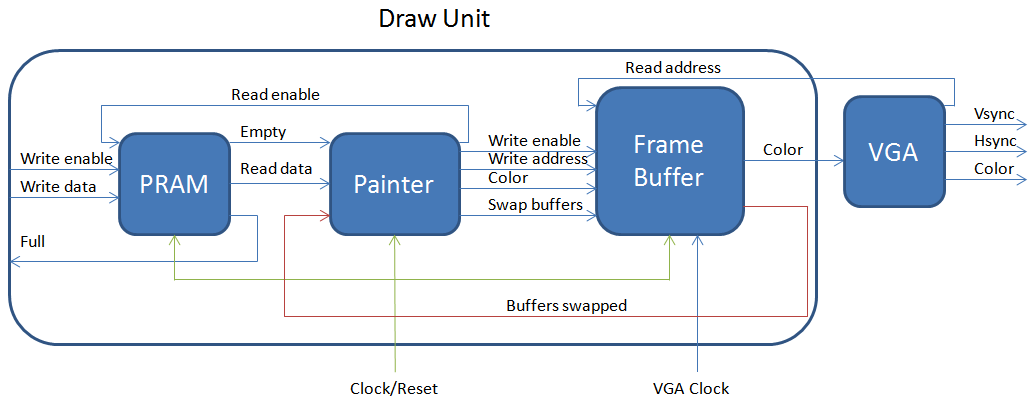
\includegraphics[width=1.0\textwidth]{draw.png}
	\caption{Draw Unit consisting of the PRAM, Painter, and Frame Buffer. VGA shown externally.}
	\label{fig:draw}
\end{figure}

The purpose of the draw unit is to write pixel colors to memory in parallel to the CPU’s calculations.  This memory, called the frame buffer, is then read by the VGA Controller, which outputs these pixel colors to the user’s screen.  The draw unit fixes the screen resolution to 160x120 to meet the block ram limitations of the Spartan-3E FPGA.

\subsubsection{PRAM}
PRAM is a memory mapped queue.  To use the draw unit, the programmer simply performs two memory writes to PRAM’s memory address.  These writes will go into the queue to be read by the painter in the order they are written.  The queue can hold up to 1024 writes.  Every two writes defines a row of pixels on the screen, a color, and the starting and ending of that row.  The first of the writes to the draw unit contains a row number and a color.  The row number is from 0 to 119 inclusive, and corresponds to the row of pixels on the monitor that should be drawn to.  This value is expected in bits 9 down to 3.  The color value is then placed in bits 2 down to 0, giving 8 possible colors.  The second memory write contains a left index and right index which define the starting and ending points of the line to fill in.  These indices can range from 0 to 159 inclusive.  The left index must be in bits 15 down to 8 and the right index is in bits 7 down to 0.  There is a single special write value, 0xffff.  When 0xffff is written into the queue twice, this indicates that the frame buffer should be swapped, which is explained in greater detail in subsection 3.

The queue is implemented using a single block ram with 32-bit addressable values, a counter, a write pointer into the ram, and a read pointer into the ram.  Since the incoming values are 16 bits, the queue is a finite state machine triggered by write enables, where the first state stores an incoming value in the upper half of a 32-bit register, and then the second state stores the next value in the low half of the register, increments the write pointer, and resets the state to the first one.  When a read enable is made, the queue simply outputs the value at the read pointer and then increments the read pointer.  Every cycle a write and/or read occurs, the count is updated (increased if only a write happens, decreased if only a read happens, or unchanged if both/neither occur).  If count is 0, an empty signal is output, and if count reaches 511, a full signal is output.

\subsubsection{Painter}
The painter reads the values out of the queue and then performs the appropriate writes to the frame buffer so that pixels have the correct colors.  It’s implemented as a finite state machine.  The initial state just checks if the queue is empty, and as soon as it’s not, sends a read enable and goes to state 2, which just disables the read enable and waits for the data from the read enable to arrive.  State 3 checks the value read from the queue.  If it’s 0xffffffff, that’s the special value which initiates a frame buffer swap.  In this case, the painter outputs the swap command as a signal to the frame buffer, then goes into a pause state because the current picture is painted and any future values in the queue are intended for the next picture, which can’t be started until the swap has been completed.  More on this is explained in section 3.

If the value read is not 0xffffffff, then the painter interprets the value exactly as was specified in subsection i.  It uses the left index and line to calculate a starting index into the frame buffer.  It then writes the specified color to that location in the frame buffer and increments the index.  This process repeats until the index reaches the address calculated by using the line number and the right index, at which point the entire line has been filled.  After some setup time, it takes only 1 cycle per pixel for the memory writes.  So if we want to fill an entire line with a new color, it takes about 160 cycles for the painter before it reads the next value out of the queue.  Meanwhile it only took the CPU 4 cycles to specify the line, color, left index, and right index.

\subsubsection{Frame Buffer}
The frame buffer is a set of 8 block rams in which pixel colors for the entire screen are stored.  There are two separate sections of the frame buffer: the front buffer and the back buffer.  The front buffer is where the VGA controller is reading from, and is read only.  The back buffer is where new pictures are drawn, and is write only.  Once a picture has been completely drawn in the back buffer, the two buffers (front and back) are swapped between a vsync so now the new picture is read-only and what gets output to the screen, and the old picture is write-only, and gets overwritten by a new one.  This prevents half-drawn pictures from outputting to the screen, and decouples the VGA frame-rate (60Hz) from the rate at which new pictures are drawn (which is variable).  This means that each pixel on the screen must have two 3-bit color values in memory: one in the front buffer, one in the back buffer.  

Since the Spartan3E only has 368kbits of usable ram, the largest factor of a 640x480 resolution that fits in this ram is 160x120.  A 160x120 resolution has 160*120 pixels, each pixel has 3 bits of color, and there are 2 copies of that pixel.  Therefore the memory used is 160*120*3*2 which equals a little over 115kbits.  Complicating matters is that each pixel is a three bit value, but only word sizes that are powers of two are addressable.  To resolve this matter, a single pixel color is stored in three different rams: one ram for bit 2 (called rbuffer), one for bit 1 (called gbuffer), and one for bit 0 (called bbuffer).  The address into these rams is then the same for each pixel.  Unfortunately, this led to each ram being 38400 bits, which is 2.34 block rams.  This meant each of the three rams wasted .66 of a block ram resource on the FPGA.  To address this, a fourth ram was created, called sbuffer.  Rbuffer, gbuffer, and bbuffer were all reduced in size to use exactly two block rams each, meaning they didn’t quite have enough room for all the pixels.  Sbuffer, using 4 bit words in which the most significant bit is wasted, contains all three bits of a color per pixel at a single address.  Sbuffer still wastes a quarter of its space, but that’s much better than the two-thirds of a wasted block ram for each of the other rams.  Figure \ref{fig:frameBuffer} displays our final frame buffer implementation:

\begin{figure}[H]
	\centering
	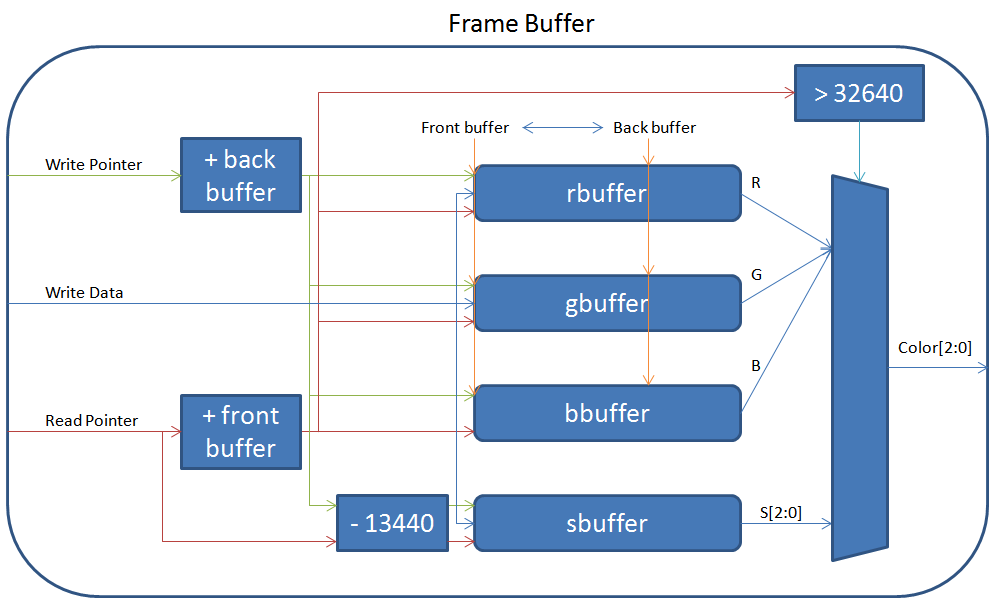
\includegraphics[width=1.0\textwidth]{framebuffer.png}
	\caption{Frame Buffer with read and write pointers.}
	\label{fig:frameBuffer}
\end{figure}

With this as our final setup, there are two very special addresses into the rams: 19200 and 32640.  19200 is the address at which one buffer ends and another begins.  The front buffer and back buffer are each simply represented by a pointer that either points to address 0 or address 19200 (represented by the orange arrows in figure \ref{fig:frameBuffer}).  When it’s time to swap buffers, those pointers just swap.  So if the front buffer initially started at 0 and then the swap buffer signal came, front buffer simply switches to pointing at 19200.  This swap cannot occur until vsync goes low, so a register is set until vsync goes low, at which point the buffers swap, and the painter then ends its pause state.  VGA always just reads at an offset from front buffer, and the painter always writes to an offset from back buffer.  The other special address, 32640, is where the rbuffer, gbuffer, and bbuffer end, and sbuffer begins.  Some simple logic inside determines if the offset from 19200 being used by the painter or VGA is above or equal to 32640, and if so subtracts 13440 from that offset and uses the result as the address into sbuffer instead of reading out of rbuffer, gbuffer, and bbuffer.

The final result of these efforts saves an entire block ram, so the frame buffer ended up using a total of eight block rams instead of nine.  Since a 3d application takes a lot of code and uses 180 bits per triangle, this meant we’d have enough memory for an extra thousand instructions or an extra 90 triangles.

\section{Assembly}
\subsection{Assembler Driver}
The assembler driver consists of three tools: a preprocessor, an assembler, and a memory padder. The assembler is written in python.

The preprocessor takes one macro called `define, which works very similar to `define in verilog, or \#define in c.   The syntax for this macro is ''`define A B``. It will then take every instance of A in the document, and turn it into B.  This is especially useful because the CPU uses memory mapped IO, which enables the programmer to simply read from a VGA macro, and have the tool convert it to the appropriate memory location.

The assembler takes the preprocessed code and turns it into instructions that can be run.  The assembly language supports several pseudo instructions, and the assembler maps those into real instructions.  The output of the assembler is a single object file which consists of a series of numbers, stored in plain text, which represent the instructions.

The final stage of the pipeline is the padder. It takes the object file produced by the assembler, and converts it into series of init text files which Xilinx can use to to place the initial data in the memory blocks on the FGPA.  This allows the programmer to quickly test the code on the board by running pad, regenerate the bit file without resynthesizing the CPU, and place it on the board.

The following is the output of a successfully assembled piece of code:

\begin{verbatim}
$ pad Program/code.asm
Preprocessing Program/code.asm
   (1/2)    Finding: [100%]
   (2/2)  Replacing: [100%]
Assembling Program/code.pp
   (1/3)   Encoding: [100%]
   (2/3) Addressing: [100%]
   (3/3)   Labeling: [100%]
Padding Program/code.o for memory of size 11264
   (1/1)    Padding: [100%]
\end{verbatim}

\subsection{Assembly Language}
The assembly language we designed takes many of it’s features from the x86 instruction set.  Although we did not design hardware with the same level of functionality in terms of compact arithmetic and address calculation, our assembler mimicked many of these features using psuedoinstructions decomposed into specialized instructions.  Other than basic arithmetic, there are a few classes of instructions worth noting which are covered in the following section.  For a full list of all of our instructions, both pre- and post-assembly, see appendix A.

\subsubsection{Stack Instructions}
The first class of x86-like instructions are the stack-based instructions PUSH, POP, CALL, and RET.  PUSH and POP write and read values in memory at the address in the stack pointer and appropriately increment or decrement the stack pointer.  These instructions were originally designed to be single cycle instructions but multi-cycle reads caused POPs to require three cycles: two for the instruction and the load delay slot and one for a separate increment instruction because structural hazards caused by the load delay slot made it difficult to accomplish the increment in the same instruction and time did not permit this inefficiency to be addressed.  On a side note, the original design of PUSH and POP led to the addition of the INCR and DECR instructions since the hardware needed to be added anyway.

CALL and RET are the other two stack-based instructions and they work like x86.  CALL pushes the return address to the stack, decrements the stack pointer, and jumps to the target address.  RET reads the value at the stack pointer into the program counter, increments the stack pointer, and jumps to the value read from memory.  These instructions allowed us very high level programming practices and code reuse through function calls and this helped streamline our development and testing of software. 

\subsubsection{Jumps and Compares}
Finding our opcode space limited to 3 bits for jump instructions, we decided to implement two compare instructions in order to avoid having twice as many jumps (i.e. just JL instead of JL and JG).  We also took this a step further by adding pseudoinstructions of the form JUMP ARG, ARG, LABEL.  The jumps can be JE, JNE, JA*, JAE*, JB, JBE, JG*, JGE*, JL, and JLE where jumps with asterisks use the reverse compare and the opposite kind of jump to perform the same behavior.  These jumps eliminated any need for the programmer to be aware of the underlying hardware and allowed the assembler to do all that work.

\subsubsection{Moves}
The last of the unique bits of our assembly code were special kinds of MOV instructions.  Wanting to emulate x86 functionality, we designed our assembler to use take move instructions of various forms: 

\begin{table}[H]
	\centering
	\label{tab:moveTypes}
	\caption{Move Instructions}
	\begin{tabular}{ c c }
	\hline
	Instruction               & Effect \\ \hline
	MOV [\%R], \%R            & Move from a register into memory at address in register \\
	MOV \%R, [\%R]            & Move from memory at address in register into a register \\	
	MOV [IMM/LABEL], \%R      & Move from a register into memory at immediate address \\ 
	MOV \%R, [IMM/LABEL]      & Move from memory at immediate address into a register \\  
	MOV \%R, [LABEL+constant] & Move from memory at a label address plus a constant \\  
	MOV [LABEL+constant], \%R & Move to memory at a label address plus a constant \\  
	MOV \%R, \%R              & Move a register to another register \\  
	MOV \%R, IMM              & Move an immediate up to 16 bits into a register \\  
	\hline
	\end{tabular}
\end{table}

All of these move instructions allowed us to easily access memory and all work determining the translation of these instructions was done transparently in the assembler.

\section{Software}
\subsection{Game Model}
%\XXX TODO

\subsection{Graphics Pipeline}
\subsubsection{Overview of a Typical Floating Point 3D Pipeline}
  The goal of a 3D graphics pipeline is to take models represented in three-space, and draw them to a two-dimensional screen.  Models are represented as a set of triangles.  These models must be rotated, translated, flattened to the screen, and drawn to pixels.  In industry standard pipelines such as Direct3D and OpenGL, these operations are performed using floating point math because there are lots of slopes and trigonometric functions.  A simplified version of the OpenGL pipeline is as follows:

\begin{enumerate}
\item Object Transformation

Triangles are translated by simple vector addition, and rotated by multiplying each point of each triangle by a matrix with the format shown in figure \ref{fig:matrices}, where theta is the rotation angle around the subscripted axis.

\begin{figure}[H]
	\centering
	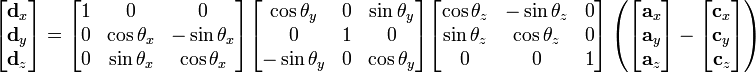
\includegraphics[width=1.0\textwidth]{matrices.png}
	\caption{Rotation Matrix. Source: %http://en.wikipedia.org/wiki/Perspective_transform
	}
	\label{fig:matrices}
\end{figure}

Note that there is one set of these matrices per model, each with different values.  These values are floating point numbers.  For object transformations, vector c is set to 0.  Vector a is the position of a single point.

\item Camera Transformation

Triangles are now rotated point-wise by a second matrix multiply with the camera matrix, again of the format shown in figure \ref{fig:matrices}.  Here vector c is the location of the camera and vector a is the current object being rotated around the camera.   There is only one camera matrix, which represents where the screen is in the virtual world.

\item Z-Clipping

Triangles behind the camera are discarded, and triangles crossing the boundary of the camera are split apart along the boundary and only the part in front of the camera is kept.  This is done using a slope-intercept calculation to generate new points along the boundary.

\item Projection Transformation

Triangles are now flattened with matrix operations of the format in \ref{fig:projectionMat}:

\begin{figure}[H]
	\centering
	%
\includegraphics[width=1.0\textwidth]{projectionMat.png}
	$$b_x = (d_x - e_x)(\frac{e_z}{d_z})$$
	$$b_y = (d_y - e_y)(\frac{e_z}{d_z})$$
	\caption{The matrix operations to perform a perspective transform. Source: %http://en.wikipedia.org/wiki/Perspective_transform
	}
	\label{fig:projectionMat}
\end{figure}

This calculation is performed for each point.  d is a point’s location vector, and e is the camera’s location vector.  b is the point after being projected.  This transformation flattens all the points to the screen location (normally z = 0).
\item Screen Clipping

Similarly to Z-clipping, triangles off screen are discarded, and triangles crossing the boundary of the screen are split apart along the boundary and only the part within the screen is kept.  This is done using a slope-intercept calculation to generate new points along the boundary.

\item Rasterization

The pixels bound by a triangle are filled in with the color of that triangle.  This is performed using the scanline algorithm.  Essentially, the screen is split up by lines.  Then for each line of pixels, the intersection of that line with a triangle is calculated.  Finally, all pixels between the two end points on a line are filled in.  See figure \ref{fig:rasterization}:

\begin{figure}[H]
	\centering
	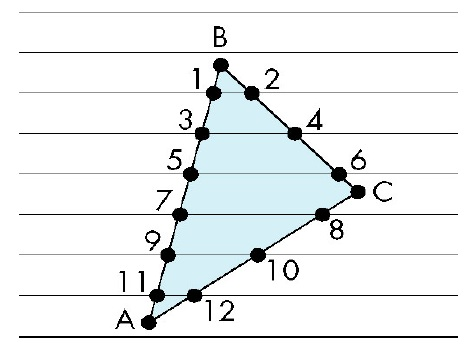
\includegraphics[width=0.50\textwidth]{rasterization.png}
	\caption{Scanline Algorithm. Source: %http://www.techfak.uni-bielefeld.de/ags/wbski/lehre/digiSA/WS0607/3DVRCG/Vorlesung/13.RT3DCGVR-vertex-2-fragment.pdf
	}
	\label{fig:rasterization}
\end{figure}


Since triangles can be layered, only the closest one to the screen should be drawn.  To do this, a buffer containing the z value of each pixel is created.  When a pixel is being drawn, the z-value for the triangle at that pixel is compared to the one in the z-buffer.  If the z-value in the buffer is farther away, then the triangle fills that pixel and the z-buffer is updated with the new, closer z value.  Otherwise, the pixel is not refilled and the old z value is kept in the z-buffer.  This completes the graphics pipeline.  In the following sections, we describe our implementation using fixed point numbers and integer instead of floating point.

\end{enumerate}

\subsubsection{Coordinate System}
We chose a coordinate system in which z is forwards, -z is backwards, -y is up, y is down, x is right, and -x is left.  Up being in the negative y direction may seem counter-intuitive, but VGA starts drawing from the top of the screen down to the bottom, so y increases as VGA goes down.

\subsubsection{Model Movement}
The first stage of our graphics pipeline starts by making a copy of the base model on the stack.  This is important as the fixed point calculations have inherent precision loss which would lead to permanent degradation of the model data if the original was not preserved.  Once the data is copied, we rotate the model.  Since it is centered around the origin, this is a simple rotation around the “up” and “right/left” axes.  This is accomplished by multiplying the first two rotation matrices in \ref{fig:matrices} by each point of every triangle in the model.  Since we lack the hardware to do a sin or cosine, we instead implemented these as lookup tables.  Since angles are naturally modular, we simply have 0x0 represent 0 degrees, and 0xffff represent the maximum angle (roughly 359.9 degrees) with a linear grade for all angles in between.  After the model is properly rotated, the next step is to translate the model to its position which was set by the game model calculations.  This is simply a vector addition to each point in every triangle in the model.

\subsubsection{Camera Movement}
Once the model is in place in the world coordinate system, it needs to be moved into the camera coordinates.  This calculation uses the same rotation matrices from the model rotation, but applies the rotation of the camera such that models are rotated to where the z-axis is parallel with the camera’s line of sight.  Since all points are already translated away from the origin, this transform essentially rotates every point in the world around the camera.

\subsubsection{Culling}
An important process in both the display of triangles on screen and the speed of rendering is to ignore all triangles which are not “facing” the camera.  That is, all of the triangles on the back side of a 3D shape or any triangles whose points are ordered counter-clockwise relative to the camera.  In this case, the triangle should simply not be rendered.  This process is called backface culling.  In our implementation, triangles which were facing the wrong way in the model had their colors set to 0xFFFF (an illegal color value).  Then, any triangle with a color other than 0xFFFF would be copied into a new temporary model and sorted for drawing.

\subsubsection{Sorting}
When triangles overlap, a determination must be made of which one is closer to the camera, and only that one should be drawn.  Since we didn’t have the memory space required for a z-buffer (it would take 160*120*16 bits), we implemented Painter’s Algorithm instead.  Painter’s Algorithm simply sorts all triangles from furthest to nearest, then draws the furthest ones first.  This means closer triangles overwrite further ones, leading to a correct final image.  From here on out triangles pass through the pipeline one at a time.

\subsubsection{Z-Clipping}
In OpenGL, this step is performed after perspective transform.   However, we can’t represent our points in the range [-1,1] because our 16-bit fixed point notation is not that precise, and we do not have a divide operation so we cannot easily rescale things into that range.  So instead, we leave our numbers as integers.  We then just check every point of each triangle to see if any have a negative z coordinate (meaning it’s not visible because it’s behind the camera).  If any z coordinates are negative, we discard the entire triangle because we designed our application so no triangle would ever be partially in front and partially behind the camera.

\subsubsection{Perspective Transform}
We avoid using matrix operations for our perspective transform because that requires a divide operation.  Instead we perform our perspective transform according to figure \ref{fig:perspectiveTransform}:

\begin{figure}[H]
	\centering
	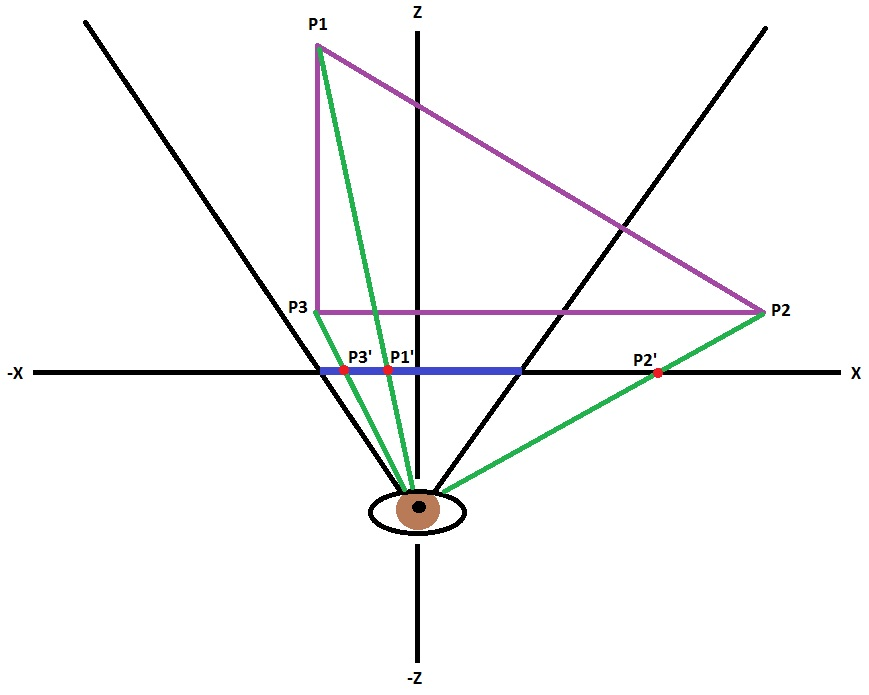
\includegraphics[width=1.0\textwidth]{perspective.png}
	\caption{Perspective transform from a top-down view.}
	\label{fig:perspectiveTransform}
\end{figure}

The eye is situated at (0,0,-100) from the screen.  This represents the user’s eye.  The screen is centered around (0,0,0), drawn in blue.  To make the triangle perspective-correct, for each point, we take the edge (represented by green) formed by the eye at one end and the triangle’s vertex at the other.  Then we find the intersection of this line with z = 0, represented by the red points.  Since we don’t have a divide operation, we can’t just use slope-intercept to calculate an intersection.  Instead we do a binary search; we keep guessing where the z intersection is until our guess has a z-value of zero.  See figure \ref{fig:binarySearch}:

\begin{figure}[H]
	\centering
	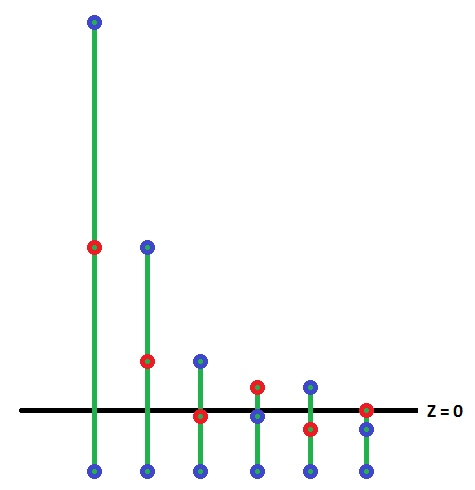
\includegraphics[width=0.75\textwidth]{binarySearch.png}
	\caption{Binary search for z = 0.}
	\label{fig:binarySearch}
\end{figure}

On each iteration, we take the z difference of the end points (represented by blue), then divide that by two.  Then we add or subtract that value to the top point based on if the top point is negative or positive and this gives us a new top end point (represented by red).  For each time we divide the z difference by two and add/subtract, we apply the same operations to the x and y value value of the point.  This ends up performing the same operation as a slope-intercept calculation only using right arithmetic shifts.  After doing this for all triangles, we have a flattened set of perspective-correct triangles.  Because the real center of the screen is at pixel (80,60) in our 160x120 screen, we add 80 to the x coordinate and 60 to the y coordinate.  Since z=0 for all points now, we can simply discard z coordinates for the remainder of the pipeline.

\subsubsection{Screen-Clipping}
Now the problem is that we have some points that are above, below, to the left, or to the right of the screen boundaries.  We can only rasterize a triangle if it’s completely within the screen boundaries.  To deal with this, we define four zones: above, right, below, and left.  Any point can be in one, two, or no zones.  If it’s in no zones, that means the point is within the screen boundaries.  If all three points of a triangle are not in a zone, then the triangle can be rasterized.  If all three points are in the same zone, it means the triangle is completely outside the screen and the triangle can be discarded.  Otherwise, the triangle is split into multiple sub-triangles along the boundary and clip is recursively called on those subtriangles.  A single triangle might be split, and then the sub-triangles may also be split.  See figure \ref{fig:clipping} for an example of this:

\begin{figure}[H]
	\centering
	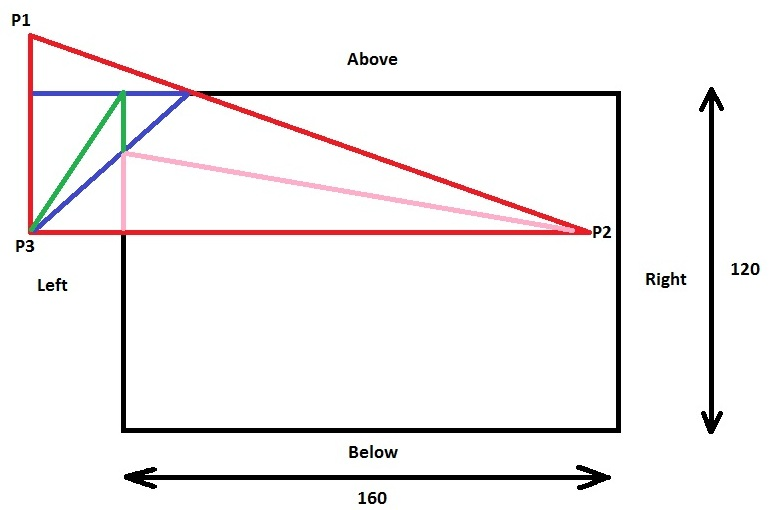
\includegraphics[width=0.75\textwidth]{clipping.png}
	\caption{A triangle being recursively split for clipping.}
	\label{fig:clipping}
\end{figure}

As seen in figure ref{fig:clipping}, we start with the red triangle.  Each point is compared with the screen boundaries to determine which zones it lies in.  Then, starting with the above zone and going clockwise, we check if any of the points are in that zone.  P1 is, so we calculate the intersection with the top of the screen using the binary subdivide helper function.  The triangle is then split along this intersection into three component triangles; the blue edges define this split.  After this, we call clip on the three new triangles.  The topmost triangle gets discarded because all three points now lie in the above zone.  The other two triangles are still partially in and partially out of the screen, so they get further split, denoted by the pink and green lines.  Eventually we end up with three triangles in which all points lie within the screen, and five triangles which have been discarded.  Each time we find a triangle completely within the screen, it is rasterized before continuing with clipping whatever split triangles remain.

\subsubsection{Rasterization}
The final step in the pipeline is to take those three points passed by clipping and determine which pixels to fill in.  Since the draw unit works on a line-by-line basis, this is how the triangle is rasterized.  We start at the top point, and work our way down one pixel line at a time.  On a given pixel line, we determine the end points of that line using a modified slope-intercept formula.  To calculate slopes, we normally need to perform division.  However, there is another way to do this: a lookup table.  In previous pipeline stages, this was not feasible due to the range of possible values (216).  But now, the range of possible y differences is [0, 119] because that’s the screen height.  Therefore we created a lookup table of 120 values, corresponding to 1/(y-difference).  Multiplying this by some x-difference gives a slope.  Rasterization proceeds according to figure \ref{fig:rasteriser}:

\begin{figure}[H]
	\centering
	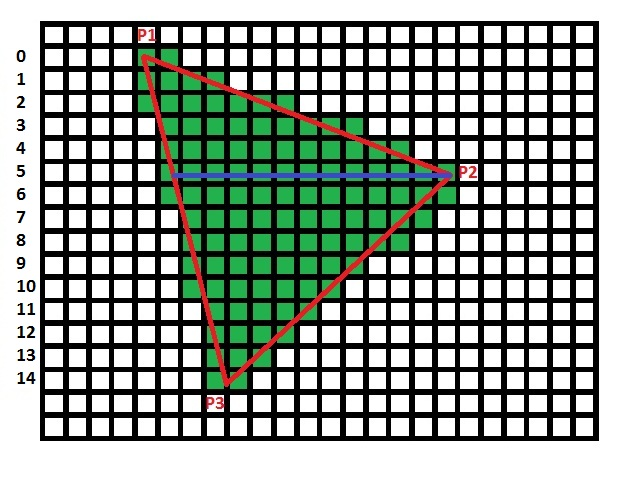
\includegraphics[width=0.5\textwidth]{rasteriser.png}
	\caption{Rasterization.}
	\label{fig:rasteriser}
\end{figure}

First the points are sorted such that the point with the lowest y-value (closest to the top of the screen) is P1.  Then P2 is the first point clockwise from P1, and P3 is the second clockwise point.  This guarantees that the edge (P1, P3) is the left bound and the edge (P1, P2) is the right bound.  Next, two incrementers, one for the left side and one for the right side, are set to 0.  Line by line, as shown by the numberings on the left of figure \ref{fig:rasteriser}, the edge pixels are calculated and then passed to the draw unit using formula \ref{eq:rasterise}

\begin{equation}
	\label{eq:rasterise}
	incrementer \times x-difference \times \frac{1}{y-difference}  
\end{equation}

The draw unit fills in everything in between the edge pixels on a line as well.  On line 5 in figure \ref{fig:rasteriser}, indicated by the blue line, there is a complication because edge (P1, P2) ends and edge (P2, P3) begins, so the slope of the right side needs to be recalculated, and the right incrementer must be reset.  There are a few other special cases, such as when the left bound is formed by two edges instead of the right bound, or when a triangle has a flat top or bottom.  Each of these is checked to make sure the correct side has its slope/incrementer recalculated.  After this point, we proceed until we reach line 14, at which point the entire triangle has been rasterized.  One additional complication arises with this method, illustrated in figure \ref{fig:rasterizerProblem}:

\begin{figure}[H]
	\centering
	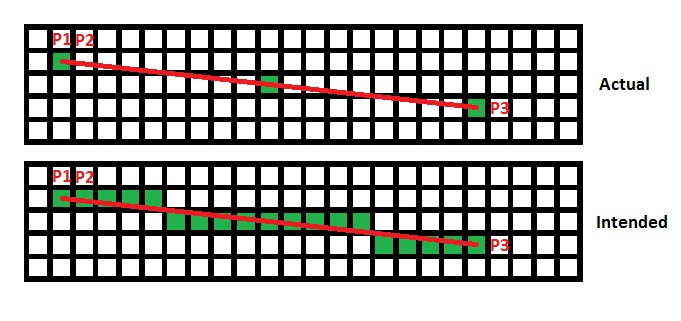
\includegraphics[width=0.5\textwidth]{rasterizerProblem.png}
	\caption{Problem with rasterization when only using endpoints.}
	\label{fig:rasterizerProblem}
\end{figure}

When a P1 and P2 of a triangle are equal, or even when the triangle is just very narrow, the above problem occurs.  The endpoints on any given line of pixels are equal, and so only a single pixel gets drawn per line instead of a connected line.  To solve this, we calculate six values per line instead of two: the two endpoints of the current line, the average of the current endpoints with the previous endpoints, and the average with the next endpoints.  Then we compare all three right points and choose the right most.  We choose the left most of the three left points.  These two points are what we pass to the draw unit, which gives us the intended rasterization.  This step completes the entire 3D pipeline.  

\section{Trials and Tribulations}
\subsection{Memory Reads}
As previously discussed in the Datapath section, memory reads are multi-cycles and utilized load delay slots.  Our original design latched memory reads halfway through a cycle rather than at the end of the cycle.  Not only did this cause synthesis to raise warnings, but also this increased the time required for the the first half of the cycle and would have resulted in half of our current 25 MHz clock speed.  Our final design successfully used delay slots and forwarding to accomplish the same goal.

\subsection{Stack}
Part of our design goals included having x86-like instructions such as PUSH, POP, CALL and RET.  All of these instructions depend on the existence of a stack pointer and management of the the stack.  We had an off-by-one error where the stack pointer would always point to the address one word lower in memory than the last thing that was pushed (either by PUSH or CALL).  But the the instructions that read from memory at the stack pointer (POP and RET) would not read the value at the address one word higher in memory where the data they were expecting resided.  On top of this, using the stack for temporary storage would result in the stack pointer being used to point to memory that would be overwritten by PUSH or CALL instructions.

Our final solution was to increment and decrement the stack pointer whenever we popped or pushed, respectively.  This follows the x86 stack convention.

\subsection{Keyboard Controller}

%\XXX TODO
 
\subsection{Block Ram Usage}
Since a 3d game takes a large code-space, a large heap for models, and a large stack for drawing those models, we designed our system to utilize all 20 available block rams on the Spartan3E.  Unfortunately, when asked for an 18 wide by 11264 tall (11*1024) ram, Xilinx ISE comes up with a frustrating optimization: it splits the ram into 18 separate 1 bit wide rams because that reduces the latency and area in LUTs.  Unfortunately, this changes what should be 11 block rams into using 18.  We figured out this was happening by carefully reading through the synthesis reports.  Our solution to this was instantiating 11 block rams, each 18 wide by 1024 tall, and then writing our own wiring scheme to interconnect them into one large 11264 tall module.

\subsection{Precision}
A 3d game must use fractions at some point because slopes and sines/cosines cannot be represented in integer.  To accomplish this without creating lots of additional hardware, we chose to use a fixed point representation of Q1.14, meaning a two’s complement number with 14 fractional bits, one integer bit, and one sign bit.  This gave us roughly three decimal places of precision.  When drawing triangles, the largest accumulated error by this precision is one pixel, meaning sometimes a corner pixel doesn’t get drawn.  To avoid this problem from being visible, we designed all models such that where two triangles in a model meet, they share the same edge.  That means both triangles have the same end points along that edge.  The math to draw the triangle is deterministic, so even if it’s off by one pixel on the corner, both triangles are off by that same amount and still meet up seamlessly instead of leaving an undrawn pixel.

\subsection{Generating Mem File}
To optimize our time while coding, we set up Xilinx ISE to generate new program files without re-synthesizing the whole CPU.  To do this, we created a mem file which holds our memory contents, and a bmm file which tells ISE how to initialize the block rams with that mem file.  Unfortunately, mem files and readmemh files (our previous method of initializing RAM) have a very subtle difference; readmemh files are white-space delimited, while mem files are hex character delimited.  To figure this out, we had to dump our bit file after generating it and actually look at what went into memory.  Once we saw the problem, we simply padded each value that was not a full five hex characters with zeroes when assembling the mem file.



\section{Individual Work}
\subsection{Daniel Blakemore}
I was mostly in charge of writing and maintaining control logic and the assembler.  In maintaining control, I also maintained all top-level integration of the CPU elements since control signals continued to change meaning for almost the entire duration of the project development.  The assembler also changed as features were added to the assembly language like the aforementioned special jumps and moves.

I also wrote a few of the simple initial mathematical stages of the software pipeline including rotation, translation, and backface culling.

\subsection{Leif Andersen}
%\XXX TODO

\subsection{Jon Parker}
For hardware, I wrote the vga controller, draw unit, instantiated the DCM, and worked together with Leif on the ALU.  I also worked with Daniel to write the memory.  For software, I wrote rasterization, clipping, and perspective transform including helper functions such as a binary subdivide.  Also, using a tutorial by Paul Willoughby and another by Tyler Nichols, I set up our ISE project to generate the program files using a mem file instead of re-synthesizing the entire CPU.


\section{Conclusions and Future Work}
\subsection{Mathematical and Model Bug Fixes}
One bug that we would fix was a clipping error. When a triangle is exactly one pixel past the screen edge, it gets stretched all the way across the screen.  Another is that the binary subdivide can sometimes be off by a single pixel; while not clearly visible, it could still be improved upon.

\subsection{Keyboard Controller}
%\XXX TODO

\subsection{Game Integration}
%\XXX TODO

References [leif/jon]..l..

\end{document}